\documentclass[cn]{elegantbook}

 \newcommand{\tabincell}[2]{\begin{tabular}{@{}#1@{}}#2\end{tabular}}%使表格内可手动换行
 \newcommand\Emph{\textbf}

 \let\widering\relax

%%%%%  TimeLine preamble  %%%%%%%%%

\usepackage[utf8]{inputenc}
\usepackage[TS1,T1]{fontenc}
\usepackage{fourier, heuristica}
\usepackage{array, booktabs}
\usepackage{graphicx}
%\usepackage[x11names]{xcolor}
%\usepackage{colortbl}
\usepackage{caption}
%\DeclareCaptionFont{blue}{\color{LightSteelBlue3}}
\newcommand{\foo}{\makebox[0pt]{\textbullet}\hskip-0.5pt\vrule width 1pt\hspace{\labelsep}}

 %%%%%  TimeLine preamble  %%%%%%%%%
 
%    \newsavebox{\mybox}
    \usepackage{titlesec}%定制section的样式
    \usepackage{geometry}
    \usepackage{cite}
    
    \usepackage{varwidth}
    \usepackage[thmmarks]{ntheorem}
    \usepackage{float}%优化插图位置
    \usepackage{wrapfig}%插入图片使之被文字环绕
    \usepackage{multirow}%表内多行合并
    \usepackage{array}%表格内自动换行命令所需 \begin{tabular}{m{5cm}}
    
    % {
    %  \theoremheaderfont{\bfseries}
    %  \theorembodyfont{\normalfont}
    %  \newtheorem*{pf}{证}
     
    % }
    % {
    %  \theoremheaderfont{\bfseries}
    %  \theorembodyfont{\normalfont}
    %  \newtheorem{example}{例}
     
    % }
    \usepackage{enumerate}%定制enumerate环境
    %\usepackage{enumitem}%定制enumerate环境的序号样式
    %\AddEnumerateCounter{\chinese}{\chinese}{}%增加中文序号样式到enumerate环境,使用示例:
                               %\begin{enumerate}[label={\chinese*、},labelsep=0pt]
    \usepackage{extarrows}
    \usepackage{mathtools}
    \usepackage{amsfonts}
    \usepackage{color}
    \usepackage{float}
    \usepackage{geometry}
    \usepackage{theorem}
    \usepackage{amsmath}
    \usepackage{amssymb}
    \usepackage{ulem}%记号
    \usepackage{bm}
   % \newtheorem{definition}{定义}
    \newtheorem{thm}{定理}
 %   \newtheorem{lemma}{引理}
    \newtheorem{prop}{性质}
    \newtheorem{method}{解法}
    \newtheorem{notice}{注}
    %\newtheorem{example}{例}
    %\newtheorem{proof}{证}
    \newtheorem{cor}{推论}
    
    
    \newcommand{\tabincell}[2]{\begin{tabular}{@{}#1@{}}#2\end{tabular}}%使表格内可手动换行
    \newcommand{\mylim}{\lim\limits_{n\to\infty}}
    \newcommand\Emph{\textbf}
    \newcommand\degree{^\circ}
    \newcommand\red{\color{red}}
    \newcommand\ue{\mathrm{e}}%e的正体版
    \newcommand\dif{\mathrm{d}}%dx正体版.
    \newcommand\diff{\mathrm{D}}%D正体版.
    \newcommand\mx{\boldsymbol}%粗体.
    \makeatletter
    \newcommand{\rmnum}[1]{\romannumeral#1}
    \newcommand{\Rmnum}[1]{\expandafter\@slowromancap\romannumeral#1@}
    \newcommand{\tr}{\mathop{\mathrm{tr}}}%\trace 
    \makeatother
    
    \bibliographystyle{plain}
    
    \renewcommand\qedsymbol{\ensuremath{\Box}}
    %\renewcommand\refname{参考文献}
    
    \usepackage[pdftex, bookmarksnumbered, bookmarksopen, colorlinks, citecolor=blue, linkcolor=blue]{hyperref}%定制目录样式
 %   \geometry{a4paper,margin=1in}
  %  \pagestyle{plain}
\title{数试学习生活指南}
\subtitle{钱院学辅}

\author{程闽华,牛嘉豪}
\institute{钱院学辅}
\date{\today}

\version{1.1}
\equote{Victory won\rq t come to us unless we go to it. --- M. Moore}
\logo{logo.png}
\cover{cover.jpg}


\begin{document}
\maketitle
\tableofcontents
\clearpage
\thispagestyle{empty}

\mainmatter
\hypersetup{pageanchor=true}

\chapter*{写在前面}
\addcontentsline{toc}{chapter}{写在前面}
\markboth{写在前面}{}
首先欢迎学弟学妹们加入到数学试验班的大家庭!\par 
会想到写这份指南,是因为我们深感大学的模式,无论是学习还是生活上,都和高中有很大的不一样:一方面大学的班级概念过于弱化,小班级又过多,
各种形式的活动、通知又很繁多,此外大学的科目较高中也精深得多,这些变化势必让人感觉无所适从——面对大学的学习与生活,就像老虎吃天一样,让人感觉无处下手;而另一方面
这些困难在经历过后再回看时,感觉也不过如此,事实上也确实不过如此。\par
这样的矛盾是很不合理的。\par
在这种情况下,一些比较幸运的同学通过各种渠道认识了一些学长,通过学长的帮扶走适应的快速通道:直系学长可以指点学习上的方向,其他专业的学长可以解答生活上的一些困惑。
但剩下的绝大多数同学可能就不那么幸运了,面对纷繁复杂的大学学习生活,他们只能如盲人过河一样,在迷茫中度过前两年,
从而也把许多精力浪费在一些没有必要的事情上。\par
或许有人认为这也考验了我们获取信息的能力,但我们仍然认为,这些摸索的代价大于收获,希望这份
数试学习生活指南能引领你快速进入大学的学习生活状态,然后专注于自己真正感兴趣的并且有意义的事情上。\par
在这份指南里,我们将你可能遇到的困惑分为“学习”、“生活”两大部分,其中“学习”部分指狭义的学习,即只涉及学习本身,而不涉及与之间接相关的其他内容,并且集中在数学的学习上;
其余与学习不直接相关的内容,都放在“生活”部分。
另外还单独设置了“出国”这一部分,具体介绍试验班出国交流项目。\par
我们推荐同学们浏览一下所有的内容,这样很多时候如果遇到了里面提及的问题后可以拿来参考,并且整个文章可以给你一个大学生活的一个初步的感觉。\par


最新版本下载地址:\href{https://github.com/ElegantLaTeX/ElegantBook/releases}{Github:ElegantBook/releases}。本文将介绍本模板的一些设置内容以及基本使用方法。如果您在使用此模板,欢迎把您使用此模板制作的成品发一份给我们,谢谢!如果您有其他问题,建议或者意见,欢迎联系我们。\par

本指南使用了开源的\LaTeX{}模版—— ElegantBook, 最新版本下载地址:\href{https://github.com/ElegantLaTeX/ElegantBook/releases}{Github:ElegantBook/releases}。






\chapter{学习}
作为试验班的学生,学习自然是很重要的一环。下面先讲讲学习成绩的功利性作用。
\begin{enumerate}
 \item 从大二开始,每个学年第一个学期初,都会在专业内对上个学年进行综合素质评测(简称“综测”),其中学分绩占比占主导地位,
 并且综测排名直接决定了你是否能获得奖学金以及获得的奖学金数额;
 \item 出国读研、读博的一个硬性标准——GPA,指的也是成绩,具体地说是平均学分成绩, 即按学分加权平均。
\end{enumerate}
除此之外,你需要明确的是,成绩并不是学习的全部,它只是你学习的一部分,而且是极其表面的一部分。
极端地说,你可以考得差,但一定要学得好。其中学得好的唯一标准,便是你能把你所学的东西纳入到自己的直观中,能够随时(至少那个学期能够随时)和人讲解这些内容。


\section{学习态度}
首先,你应当去思考,来大学是为了什么,学数学又是为了什么,现在肯定还没有答案,但这两个问题希望贯穿你四年的生活,让你不断有更好的答案,当你可以给出更精彩的答案时,你的生活,你自己都会变得更加绚丽。但我要提醒的是,不要轻视或者简化这个问题。当选择数学试验班的时候,有人是立志成为数学家;有人是因为觉得数学有趣;有人觉得数学是万金油,学好了做任何事情都可以;有人因为没什么专业喜欢,先学个数学以后好转行;或者有人是因为数学试验班资源很好,有出国交流的机会,重点培养而来。我想这所有的答案都可以作为选择的依据,但不能作为度过这四年的理由。你会在此经历学业上的困难,生活上的挫折,来自未来越来越多的压力。立志成为数学家的同学可能发现数学研究并不是自己所想的,而想转行的同学可能会发现科研可能是最适合自己的职业,觉得数学有趣的同学可能会失去兴致,但对数学知识感觉一般的同学可能渐渐发现数学的惊奇。但你只有不断思考自己想在大学学到什么,想从数学中学到什么,你才能迎难而上,创造出自己的大学生活。所以学习态度不是一个别人给予的答案,不是一个我感兴趣,我不感兴趣的答案,但我依然想做一些鼓励和提醒来帮助大家去树立自己的学习态度,因为这在我们回顾已经度过的大学时光后一致认为是最为重要的。

\subsection{什么是专业——数学外的学习}
大家的专业是数学尤其是作为数学试验班的学生,学好数学自然是学习中最重要的一环,但大学学习远不止这些,这种环境,可以让你去接触一切你感兴趣的东西,经济,历史,哲学,心理,生物,物理,宇宙学,工学,舞蹈,排球等等的内容,虽然你可以从饱满的学习任务中挤出的时间很少,但我仍鼓励你可以在不影响自己主课学习的过程中去经历不同的课或者活动,结交不同的朋友。其实我们有这样的时间和机会,但如果你每次选课都在思考哪个给分高而不是了解一下具体的内涵,只在意GPA而不是自己的成长,那或许没有这样的机会和时间。所以专业是选了一个主旋律,但如果没有别的东西,那称不上精彩。

\subsection{数学的学习态度}
很奇怪的是,我先提及了非数学的学习,因为数学的学习绝对是一个复杂且具有挑战性的事情,你应当在其中有认真的态度,你应当掌握课内要求的知识,做充足的练习并且对数学积累足够的经验和感觉,训练有素是个基本的目标。但我想提醒的是,虽然我们是理科,学习内容,学习方式都是,但数学本身却又是个十分感性的学科,我希望你可以时常拿文学,哲学来类比。学文学肯定不会是去背诵文章主旨,起码大学不是,那学数学也不是单纯掌握和应用数学书上的定理和命题。你应当追求一种体系的建立,以自己的方式梳理你学过的每一门课和每一门之间的联系,这当然是在掌握课内知识的基础上,但这才是最重要的一步,因为数学是为了提高人们理解和描述概念和问题的能力,给你新的看待世界的方式,塑造你无与伦比的思维模式,而这些正是通过定理和命题这种抽象的方式而进行的,所以你需要时刻惦记着这件事。除此之外,数学的学习和上一条其他方面的学习是紧密相连的,我们通过学习数学,事实上应当学习到教育所期待我们学习的一切,我希望你们可以在学习过程中感受到,学数学不是修一门课,读一本书,证明一个命题。她是一个完整的思维奇迹,一门感性的艺术。学习数学是让抽象概念,思维方式,融入大脑的过程。这些概念会反复挑战我们的思维,进而来帮助自己更好的理解这个世界,无论是生物,物理,工程,计算机,还是经济,社会体系,甚至是哲学,心理学。数学,尤其大学里学习数学,远不是今后非要拿这些理论来谋生,即便是数学工作者,用到的只是某一专一领域中的知识。这应是一场旅程,一次受人类智慧熏陶的过程,希望数学的智慧,可以鼓舞你不断思考,反复追问,帮助你们在四年中去思考,自己将成为什么样的人,过怎样的生活。希望你可以沉浸在这样的氛围中,去结交朋友,思考问题,碰撞思维,因为这就是数学的奇妙,她让你碰到无数有趣的灵魂,难忘的经历,带来无与伦比的体验,最终引领我们自我实现。所以,当你认真对待这份值得你精力的学业,我坚信,生活的美好将会在面前自然地展开,祝你们好运!



%\newpage

\section{教材目录}
为方便学有余力的同学自学(实际上我相信每一个同学如果认真学习,也就是能做到上课认真听讲、课后认真复习、课后习题都做一遍的话,都可以做到学有余力),我们在这列出2017级数试大一到大三的数学课程教材目录。

    \begin{table}[h]   
    \begin{tabular}{c|c|c|c|c|l}
        %\multicolumn{5}{c}{16级大一大二教材目录}\\
        \hline
        \hline
        学期 & 课程名 & 教材名 & 作者 & 出版社 & 备注\\
        \hline
        大一  & 数学分析 & 数学分析教程   & 常庚哲、史济怀 & 高等教育出版社  &  \\ \hline
              & 高等代数 & 高等代数	& 丘维声	&科学出版社	& \\ \hline
              & 数论基础 & 初等数论	& 闵嗣鹤	&高等教育出版社&  \\ \hline	
        大二上	&数学分析	&数学分析教程	&	&	&多元微积分  \\ \hline
               &常微分方程	&常微分方程及其应用	&周义仓	&科学出版社&\\ \hline
               &近世代数	&代数学引论	&聂灵沼, 丁石孙	&北大出版社&\\ \hline
        大二下	 &数值分析	&数值线性代数&  徐树方	&	北大出版社&\\ \hline
                &        &数值逼近	& 蒋尔雄	&复旦出版社&\\ \hline
                &拓扑学&	基础拓扑学讲义	&尤承业	&北大出版社& \tiny{点集拓扑+基本群} \\  \hline
                &实变函数	&实变函数论	&周民强	&北大出版社&\\ \hline
                &复变函数	&Complex Analysis&	Stein &	&\\ \hline
                &概率论	&概率论	&苏淳	&科学出版社&\\ \hline     
        大三上  &泛函分析  &泛函分析讲义(上册) &张恭庆 &北大出版社 &\\ \hline
                & 微分几何  & 微分几何初步 & 陈维桓 &北大出版社 &\\ \hline
                &偏微分方程 & 数学物理方程讲义 &姜礼尚 & 高等教育出版社 &\\ \hline  
        \hline
    \end{tabular}  
    \caption{17级大一到大三数学教材目录}
    \end{table}  

%\newpage

\section{数学课介绍}
首先说一下总体上的建议, 就是要多读书,多做题。并且在这两者之间要有一个平衡。具体地说,多读书一定要建立在读懂的情况下,如果没完全读懂的话,读再多书作用也不大。所以读书一定要做题。做题的量根据自己水平而定,如果课后题一下子就能看出答案那基本上不用做题了,可以读进一步的书了。如果课后题很多不会做的话,那就一定要把例题和课后习题好好做一遍。最后达到课后题基本都会做的水平,就可以读下一本书了。\par
另外,如果书里面不理解的内容非常多,那就是基础没有打扎实,建议自己检查一下哪些基础知识没学好,然后回去补(基本上数分和线代没学好就寸步难行了,这两门是最重要的基础,希望一定要重视,不然补起来就比较难了)。\par
最后,一定要重视例子。因为越是抽象的东西,有例子做支撑才能理解好。对于每个定理,都需要知道它应用的几个具体例子,那样的话至少可以达到一个初步的理解。\par
在掌握课内基础知识的内容后,很多同学会开始迷茫,不知道是学一些别的课程,还是继续做更困难的习题;是读一本书,还是找个老师做做科研训练。首先我不建议急于做很多问题,因为这个世界上有太多太多未解决的问题,而数学的目标也不是解决所有的问题。数学追求的是理解而不仅仅是答案,所以趁大学低年级间,时间比较充裕,应该更自由的接触一下数学的各个领域,而不是被困在科研问题里,限制了自己的兴趣和想法。至于接触数学的哪些方面,以什么方式接触,其实不那么重要。如果你已经发现了一个或几个使你感兴趣的领域,不妨直接想办法了解,读书,问老师,如果碰巧有志同道合的同学可以一起办个讨论班都是很好的方法;如果你还没发现,或者发现了却无从下手,我建议可以抽时间看一些数学史,最经典的就是M.Klein的《古今数学思想》,当你了解了历史,不但可以大大帮助你理解一切所学的数学课程,而且还会让你萌生对数学浓烈的情感,使你成为一个有趣的数学学习者。\par
(以下推荐的参考书都是不错的书,但是希望同学们不仅仅是想到的时候拿出来翻一下,而是要花心思好好读。如果我列了很多参考书,你没必要每本都读,但是如果要读的话就花心思读好,克服一切困难,而不是随便翻翻,结果哪本书都没明白)
\subsection{数学史}
这一块我们也不是专家,我们学校也没有专家,所以我就只推荐久负盛名的M.Klein的《古今数学思想》,还有很多像《普林斯顿数学指南》等类型的书籍中也有很多历史内容,和一些数学的典范应用,都值得有兴趣的同学们一读。了解数学的故事,了解数学家的故事,是我们大学教育缺失的重要环节,如果你学了所有的必修课,却给亲友讲不出任何数学家的故事,谈不出任何数学的趣事,学数学专业可能把你学的很无趣,但我想这些书不仅可以改变这个现状,还可以作为生活的调味剂,倒也不一定要从头读到尾,有空读几节,坚持下去!
\subsection{数学分析}
数学分析是大学里面最重要的一门课,也是学分最高的一门课,是所有分析课的基础。对此一定要重视。我建议是不仅要把书后面的题好好做一做,而且最好还能看一些课外的参考书。推荐:菲赫金哥尔茨《微积分学教程》(这本书很厚,看一部分自己需要的就行),Rudin《数学分析原理》,谢惠民《数学分析习题课讲义》(没必要全做,但是尽力做一下会有收获的)除此之外,Zorich 的《数学分析》框架比较大,把数学分析的很多内容推广到更一般的情况下来做,可以时常参考,或者等学完数学分析后进行阅读来让分析的理解上升一个台阶。数学分析曲线曲面积分与微分几何相关,可以了解外微分与stokes定理,推荐\,Munkres\,《流形上的分析》
微分学可以在简单了解赋范线性空间的基础上尝试了解无穷维赋范线性空间的微分学,这个不会比多元微分学困难,但学习后对理解会大有裨益。
\subsection{高等代数}
高等代数是大学代数里面最重要的课,也是所有代数课的基础。不管是在哪个领域都是很重要的工具。丘老师的书内容很多,习题也很多,我建议主要把他布置的习题做了,没必要所有题都做,不然的话会花太多时间。然后除了丘老师的教材,还可以找几本参考教材(北大蓝以中的高等代数教材是不错的参考),学习一下不同老师的风格,比较一下证明的异同,会理解更深入一点。\par
还有就是,这门课一定要勤于计算,并且证明要反复读。因为代数的证明可能会比数学分析的证明难懂一点,所以需要自己拿几个例子好好算一下,并且反复看证明。\par
另外,学有余力的同学还可以自己思考一些问题,比方说把线性代数的结果推广到除环或者主理想整环上会怎么样?


\subsection{数论}

数论有一定难度,但是初等数论里面很多内容是和近世代数紧密联系的。学的时候建议自己学一点简单的近世代数,两者结合可以理解更深刻。
比方说研究\,$\pmod{m}$\,就是在一个循环群里面研究,原根的存在性就是说的\,$(\mathbb{Z}/m\mathbb{Z})^*$\,是循环群。
比较难的是二次互反律,一般对证明不做什么考察要求,但是如果对此感兴趣的话,可以去看看\,Serre\,数论教程的第一章,利用有限域对这个的一个诠释,是很有趣的。另外,二次互反律更进一步的发展在代数数论里面,这个理论是比较难的,但是有兴趣的话可以在之后学学,需要一定的\,Galois\,理论和交换代数基础。

\subsection{常微分方程}

在计算方面好好算一些例子,在证明方面主要考察的还是数分,所以数分一定要学好。\par
如果想对常微的理论作更深的了解,可以阅读李承治老师的《常微分方程教程》,由于李老师本人是分支理论的大师,所以里面不仅对解的存在唯一性定理作了更细致的讲解,也包含了许多定性理论和分支理论的内容,这也是所谓“动力系统”中的内容。\par
如果对分支理论很感兴趣,可以进一步阅读李老师和我们学校马知恩、周义仓老师合著的《常微分方程定性与稳定性方法》,也是一本起点比较低、讲解比较透彻的比较亲民的好书。常微分方程有深刻的几何内涵,阿尔诺德 的《常微分方程》是很好的著作。更深入的内容内容可以在学完微分流形和复变函数后接触。

\subsection{近世代数}

近世代数同样也是是一门比较难的课,很多东西是全新的。建议自己要按着书上把基本性质好好推一遍。一开始遇到题不会做也很正常,不要害怕看答案,做不出来的习题当做例题,当例子足够多了之后,就会适应抽象的语言,遇到问题甚至会情不自禁的抽象化处理。考试时这门课对大家要求反倒是不高,参考课本和丘维声《近世代数》(有习题解答)即可。但如果是想对这一门课有更系统的了解的同学,我们推荐参考书:Rotman《群论导论》(前几章就够了),GTM167《域论和Galois理论》(证明很详细),冯克勤《近世代数引论》,推荐大家了解一下范畴论中最最基本的概念(Wiki百科上就够了),因为范畴论是集合论之后又一大语言革命,如果说集合论是把一切看成集合,那么范畴就是把一切看成所谓的“态射”,范畴的语言已经成为代数学与几何学的基本语言,它不仅可以让你更系统的思考抽象代数,更会给你的思维方式天翻地覆的变化。温馨提示:范畴论就像集合论一样,必须了解,但如果太深入,反倒是有些浪费时间。最后提及一些李文威编写的《代数学方法》,是新出的好书,但观点很高难度很大,对代数有兴趣的同学可以拿来参考。

\subsection{数值分析}
主要考察线性代数和数学分析的知识,但其中很多内容的思想在代数,组合,数论,泛函分析都会遇到,所以大家应该对这门相对轻松的课程抱有认真的态度。
\subsection{拓扑学}

我们教材(用的是尤承业老师的书)题量不是太大,而且有提示,建议基本上做一遍。点集拓扑部分推荐\,Munkres\,的拓扑学。代数拓强烈推荐A.Hatcher的《algebraic topology》第零章的内容,学习了CW复形后,你会发现你的几何世界变得截然不同,除此之外,Armstrong的《基础拓扑学》里面有很多课本中内容不同的讲法,图文并茂,引人入胜。温馨提醒:几何的灵魂在于生动的例子,不要困在复杂的定义中,当你真正用心去学习上面所提到的几何的内容,你会发现儿时一切的想象在此完整的实现。\par


\subsection{实变函数}

推荐接触抽象测度论,抽象测度论的方法和传统实分析截然不同,用测度思考,可以把很多问题变得简单明快,真正理解现代分析的力量。抽象测度论也是学习概率论的基础,在学习抽象测度论后,概率论的学习将变得势如破竹。书籍推荐:胡适耕《实变函数》,Cohn《Measure Theory》(很厚,用于参考,未来从事概率或者统计方向的同学,可以抽假期细致的学习一遍),Folland《Real Analysis》(观点很高,不妨在实变函数课后期和泛函分析课程学习中拿来参考)


\subsection{复变函数}
这门课非常好,可以学到很多有用而且有趣的东西。希望大家能喜欢上这门课。教材是\,Stein\,的复分析,里面有很多理论和应用,题目质量也很高,老师推荐的参考书是方企勤《复变函数》写的更接近中国风格,也和考试更贴近,所以建议大家多参考这本书,但注意前三章的内容不是重点却并不简单,一开始可以简单翻阅,不要恋战。另外,龚昇的复分析也不错,是一本好的参考书(不过也不简单)。大家学习的时候要注意里面的几何理论和PDE的理论。这门课是黎曼面和PDE的很好的预备课。
\subsection{概率论}
与实变关系密切,但是一般本科课程不会从完全严格的实变的基础开始讲,而是更加注重应用,但有兴趣的同学一定要在很好学习抽象测度论后严格化书上所有的证明,会让理解再上一层。难点是极限定理和一部分比较难的概率的计算。中心极限定理和大数定律的证明建议好好看一下,这个非常重要,并且主要还是数分知识。前面的古典概型会涉及到一些组合知识,虽然技巧性很强但要求并没有那么高,好好做一下题应该能应付。

%\newpage

\input{./subfile/study_others}
%\newpage



%\newpage


\chapter{生活}

\section{食宿网行}
    \subsection{校园地图}
   % \paragraph{注}
    \begin{enumerate}
        \item 下面要谈及的重要地点已经用橙色标注出来;
        \item 这份地图版本比较老,图中的西食堂已变为梧桐苑,其西北侧的“拟建大学生文体中心”已建成,我们非常鼓励你去里面健身、打羽毛球、乒乓球等。
    \end{enumerate}
   
   \begin{figure}       
        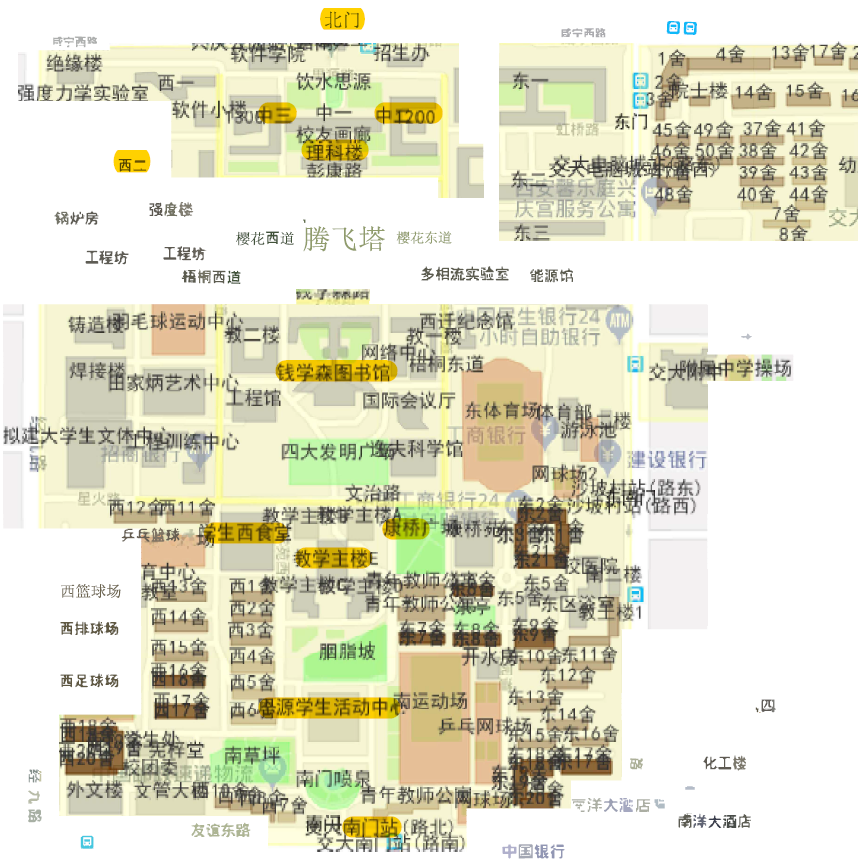
\includegraphics[scale=0.7]{./picture/map.png}     
        \caption{校园地图}
        \label{map}  
    \end{figure}    



    \subsection{饮食}
        \subsubsection{食堂}
            食堂里种类还是蛮丰富的,凭记忆列举必然挂一漏万,所以这里也不求全,这列举大概的品种让你有个初步印象,余下的就请你自己摸索啦!\par
            另外,整体而言,康桥比梧桐便宜一点
            \begin{table}[h]
                \begin{tabular}{c|p{7cm}|p{7cm}}
                    \hline
                    \hline
                         &  康桥   &  梧桐  \\ \hline
                    位置 &  见图\ref{map} &  见图\ref{map} \\ \hline
                    一楼 &  \tabincell{c}{早餐:包子,各种饼,豆浆牛奶,汤圆,\\鸡蛋,粥\\午餐:快餐,各种面,苗香掉渣饼} 
                            & \tabincell{c}{早餐:包子,油条,豆花,豆浆牛奶,粥\\午餐:鸡排饭、砂锅拌饭、黄焖鸡米饭,\\各种面;水吧、果吧}\\ \hline
                    二楼 & \tabincell{c}{自选,各种点心,各种面(有实惠的\\三块七,手头紧张的时候可以缓解经\\济压力)}
                            & \tabincell{c}{自选,各种点心,各种面(有实惠的三\\块五的面),奶茶,饺子}\\ \hline
                    三楼 & \tabincell{c}{各种又贵又好吃的}   & \tabincell{c}{各种又贵又好吃的(清真餐厅、教工\\餐厅、西餐厅)}\\
                    \hline
                    \hline     
                \end{tabular}
                \caption{两个食堂各楼层粗略介绍}
                \label{shitang}
            \end{table}

        \subsubsection{夜宵}
            夜宵出摊的时间不固定,甚至是否出摊也没有规律(主要取决于城管的心情),但一般来说还是建议最早在晚上十点左右去买夜宵;另外,吃夜宵对身体不太好,应少吃哦。
            \begin{enumerate}
                \item 南门:熏肉大饼,杀马特小哥炒细面,烤冷面,炸鸡,烧烤,臭豆腐等等
                \item 东南门:熏肉大饼,小笼包,烧烤,章鱼小丸子等等
            \end{enumerate}

        \subsubsection{聚餐}
            权当抛砖引玉吧,我们也没有去过多少地方。
            \begin{table}
                \begin{tabular}{c|c|p{3cm}|p{3cm}|p{2cm}|p{3cm}}
                    \hline
                    \hline
                          &  店名  &  位置   & 优点   & 缺点   & 备注  \\ \hline
                    炒菜  &  九龙  &  南门口  &  相对便宜,也挺好吃  &  吃多了会腻 & 有烧烤  \\ \hline
                          & 外婆印象 & 东南门外沿北直行,华润万家对面,屈臣氏旁边电梯上二楼 & 相对便宜,好吃 & & 很划算,力荐 \\ \hline
                    风味小吃 &  黄焖鸡米饭  & 南门口  & 挺好吃,有辣度  &  偏贵,人多   &  \\ \hline
                    烧烤  &  老赵烤肉 & 南门一直往南走 &  味道还行 & 偏贵  & \\ \hline
                         &  兰州拉面 & 南门口  & 挺好吃,相对便宜 & 种类偏少  &  \\ \hline
                    自助 &  千家粗粮王 & 东南门外沿北直行,华润万家对面,屈臣氏旁边电梯上三楼 & 相对便宜,也挺好吃 & 吃多了会腻,不适合很多人 &  \\ \hline
                         &  鑫海汇  &  立丰  &  海鲜为主,酒类也较多  &  偏贵  &  \\ \hline
                    火锅 &  重庆老板火锅 & 南门口西行 & 种类多,有辣度,挺好吃 & 贵  & \\ \hline
                         &  龙之秀  & 南门口西行  &  相对便宜,有大包厢  & 店比较小  & 中秋会送月饼,平时也可能会碰上变脸表演\\ \hline
                    串串  &   & 东南门外一条街   & & & \\ \hline    
                \end{tabular}
                \caption{聚餐地点粗略推荐}
                \label{jucan}
            \end{table}

    \subsection{水电费}
    \begin{enumerate}
        \item 找宿管阿姨联系租空调;
        \item 空调电费与其他电费独立,都在康桥一楼西北门的窗口交;
        \item 照明电余量不多(大概还剩五度电)时,宿舍会自动断电,这时找宿管阿姨开电即可,当然要尽快交电费,因为5度电大概只能用2-5天。
        \item 空调电24h供应,熄灯后照明电会断电。
    \end{enumerate}

    \subsection{上网}
    在学校里,上网方式主要分为两种——“宿舍有线网”和“校园Wi-Fi”。为方便起见,我们把宿舍的有线网称为“校园网”。
    \subsubsection{校园网}
    \subsubsection{校园Wi-Fi}
    见表\ref{wifi}
        \begin{table}[h]           
            
            \begin{tabular}{c|c|c|c}
                \hline
                \hline
                名称 & 有信号的地方 & 资费 & 登陆方 + 密码)\\ \hline
                XJTU\_STU & 教学区\footnote{即上课的地方,如主楼、中二、中三等} 及附近的过道 & 20元每月 &netid\verb!@!stu + 校园网密码\\ \hline
                xjtu\_lib  & 图书馆  & 免费  & netid\verb!@!xjtulib + 校园网密码\\ \hline
            \end{tabular}
            
            \caption{校园Wi-Fi}
            \label{wifi}
        \end{table}
%\newpage
       
\section{自习场所}
建议不要在寝室学习,寝室最好是用来放松、休息的地方。寝室之外有很多自习场所,现列表如下:
\begin{table}[h]
    \begin{tabular}{l|p{3cm}|p{3cm}|p{3cm}|p{3cm}}
        \hline
        \hline
        楼名   & 位置  & 优点    &    缺点  &  备注\\ \hline
        图书馆 & 学校正中心             &可连图书馆WiFi,随时可以拿馆内书籍,方便查文献;有插座的位置多,方便给手机充电
                & 预约制执行力欠缺,体验不好 & 建议提前预约,如果遇上有人坐了预约的位置,建议请走对方\\ \hline
        主楼  & 学校中轴线上,图书馆南边,思源活动中心北边,康桥西边,梧桐东边 &位置多,空间大,离宿舍近
                & 人多,可能会比较吵;期中期末考试期间可能很多教室被作考场  &  去之前可以上西交link、ehall等查空闲教室\\ \hline
        中二、中三\footnote{全名为中心二楼、中心三楼} & 分别在理科楼东边、西边 & 安静、人少、教室多 
                & 离宿舍太远    & 同上,建议先查好空闲教室 \\ \hline
        西二  &  中三西边,学校西北角,机械学院的楼;自习场所在三楼  &  人非常少,可以一人用一间教室,写黑板辅助思考等;教室的插座也可用于充电 
                & 离宿舍太远    & 随时可以去 \\
        \hline
        \hline
    \end{tabular}
    \caption{校内自习场所}
\end{table}
%\newpage

\section{出国交流}

\subsection{交流项目介绍}
    这里所列举的交流项目是目前已经确定的交流项目,仅供参考,具体若有改动,还以学院通知为准。
\begin{table}
    \begin{tabular}{c|p{3cm}|c|p{3cm}|p{3cm}|p{3cm}}
        \hline
        \hline
        年级  &  学校  & 时间  &  优点  &  缺点  &  费用\\ \hline
        \tabincell{c}{ \\\\大一\\大二} & \tabincell{c}{ 加拿大\\阿尔伯塔大学\\(10人)} & 7月初-8月初  
                & 可以提前适应西方的学习生活,为大三的交流作准备 & 时间较短,不容易沉下心学习 & 除去报销费用后,个人花费一般不到一万人民币\\ \hline
        大三下 & 新加坡国立大学NUS(3-5人) & 1月初到5月初 & 学校排名较高,有安排导师 &  &   \\ \hline
                & 密歇根州立大学MSU(10-15人) &     & 数学专业较强,数学课全,安排导师,接待周到,费用低 & 学校排名相对较低  &  \\ \hline
                & 佐治亚理工大学GT(10-15人) &     &动力系统方向较强,有安排导师 & 住宿环境可能不太好 &  \\ \hline
                & 加州大学伯克利分校UCB(3-5人) &   & 学校排名较高,数学专业强势 & 很难找导师,费用高 & \\ 
                \hline
                \hline
    \end{tabular}
    \caption{交流项目简介}
    \label{ex-pro}
\end{table}


\subsection{材料}
\begin{enumerate}
    \item \Emph{护照:}应尽早办好,有效期十年;需要本人到当地区县级以上公安局办理,需要十个工作日。
    \item \Emph{visa信用卡副卡:}在银行办理以父母信用卡为主卡的副卡,需要本人。办副卡是最理想的方案,
                        直接用主卡可能会出问题(非持卡人刷信用卡可能会遭到拒绝),但如果实在来不及办副卡,
                        建议在你在信用卡背面签上你父母(持卡人)的名字,刷卡需要签名时,也签上你父母的名字即可。
    \item \Emph{签证:}确定交流名单后,即可着手办理,其中,签证需要材料如下:
        \begin{enumerate}[(1)]
            \item \Emph{护照}。
            \item \Emph{财产证明:}银行六个月内流水(不宜过多也不宜过少,建议专门开一个账户,存款一万-十五万);行驶证;房产证明。
            \item \Emph{家庭成员身份信息:}户口本复印件(如与父母不在一个户口本上,应出示出生证明)、身份证复印件。
            \item \Emph{父母在职证明:}加盖单位公章。
            \item \Emph{父母单位营业执照复印件}。
            \item \Emph{校方邀请信:}学院会发。
            \item \Emph{与护照一致的照片:}一致指的是书否戴眼镜、是否扎头发。建议在公安局拍护照照片时,带上u盘拷电子版,
                        以后需要时打印照片即可;当时没有拷的话,也可提前抽空拍一张一致的照片,同时索要电子版,
                        以后需要证件照时只需打印,无需费力找照相馆。
            \item \Emph{签证资料表:}在大使馆官网上可下载。
        \end{enumerate}
    \item \Emph{保险:}签证办好后,便可联系买保险的事宜。
\end{enumerate}

\subsection{出国应携带的物品}
    \begin{enumerate}
        \item \Emph{证件:}护照、身份证(非必需)、邀请信(电子版即可,打印也行)、签证(在护照内)、学生证、机票。
        \item \Emph{随身品:}少量当地货币(非必需)、visa信用卡、银联卡(在具有银联标识的atm机上可直接取现金)、路上的零食、纸巾、水杯。
        \item \Emph{电子产品:}手机、电脑、相机、各种线、耳机、鼠标、当地电源转换器(加拿大和美国都是美标)、U盘、移动电源。
        \item \Emph{学习用品:}书、笔、纸、本子。
        \item \Emph{生活用品:}衣物、洗漱用品、毛巾、拖鞋。
        \item \Emph{乱七八糟:}自拍杆(合影神器)、电池、泳衣泳镜。
        \item \Emph{厨房用品:}酱油、蚝油、调料盒、盐(米可以不用买,至少加拿大的米不贵;这些东西可以一伙人各买一点)、电饭煲\&变压器
                    (手机、电脑的插头自带变压,但电饭煲的不一定自带变压,如果没有一定要带变压器,不然米煮不熟)、保鲜膜。
    \end{enumerate}
%\newpage

\section{遇到意外情况怎么办}
\subsection{身份证丢了怎么办}
首先不要慌,什么事情都是可以解决的。\par
如果不急着用身份证,即使不是陕西人,也可以带上护照、学生证、户口本中的任何一个,直接到学校东南门外那条美食街上靠北的“碑林区沙坡村派出所”异地补办身份证,一个月之内就能办好,具体工作人员会通知,短的话可能十个工作日就能办好。\par
如果急着要用身份证,比如取火车票,可以提前到火车站,办理临时身份证明,具体到火车站询问工作人员即可,如果自带近期一寸照片,全程两三分钟即可办好。另外,火车票和机票是可以用护照购买的,只是这样购买的火车票只能在柜台取。\par
此外,还可以让父母到户籍所在地派出所申请办理“临时身份证”,这不需要本人,而且只需要提供近期一寸照片即可,而这只需在可以拍身份证证件照的照相馆拍照后,要求给一份电子版的照片,然后发给父母,带到派出所即可。
\subsection{打游戏}
很多人一上大学,以为十二年的学终于上到了头,可以好好放松一把。结果夜夜笙歌,沉迷游戏,最终门门灯笼高高挂,甚至在退学的边缘反复试探。游戏或者说任何一种纯粹的消遣方式,如果适度并且可以缓解紧张的生活节奏,我想都可以接受,但如果将你的生活变得一团糟,让你的前路变得迷茫,甚至让你无所事事,最终继续消遣,那这种消遣可以认定为精神毒品。利用短暂的大学时光,思考如何更好地完成了当下所有的学习任务,思考未来想做什么事情,想成为什么样的人,会是更加意义非凡的。
%\newpage



\chapter{出国}
\section{阿尔伯塔UA}
加拿大的阿尔伯塔大学(University of Alberta,简称UA)基本上将是你出国交流的第一站,
时间不长,大抵五周,而且课程也大多是专题介绍的形式,课程尽管有一定难度但时间安排并不紧张,
所以学习压力并不大,除学习之外,体验生活也是很重要的一环。

\subsection{课程简介}
根据2018年的情况,开设的课程有 Short Courses,Special Talks 和 Special Tutorials,其中一课时指一节2小时的大课,Talk 指讲座。

\subsubsection{Short Courses}
\begin{enumerate}
    \item \Emph{最优传输理论简介(An Introduction to Optimal Transport)}(2课时)
    \item \Emph{复合矩阵与微分方程(Compound Matrices and Differential Equations)}(3课时)
    \item \Emph{网络中的动力系统:从传染病到无人机(Dynamics on Networks: from Epidemics to Flight of Drones)}(3课时)
    
    \item \Emph{统计机器学习(Statistical Machine Learning)}(2课时)
    \item \Emph{浅尝动力系统(A Taste of Dynamics)}(2课时)
    \item \Emph{从二项式模型到Black-Scholes公式(A tour from the binomial model to the Black-Scholes formula)} (2课时)
    \item \Emph{小波变换及其应用简介(An Introduction to Wavelets and its Applications)}(2课时)
    \item \Emph{什么是几何分析?(What is Geometric Analysis?)}(3课时)
\end{enumerate}

\subsubsection{Special Talks}
\begin{enumerate}
    \item \Emph{共形场论(Conformal Field theory)}
    \item \Emph{代数几何(Algebraic Geometry)}
    \item \Emph{时滞微分方程简介(A Brief Introduction to Delay Differential Equations)}
    \item \Emph{生物复杂性和动力系统(Biocomplexity and Dynamics)}
\end{enumerate}

\subsubsection{Special Tutorials}
\begin{enumerate}
    \item \Emph{Matlab}
    \item \Emph{\LaTeX}
\end{enumerate}


\subsection{饮食}
在外面吃快餐平均一餐10加元左右,其中整体上而言,肯德基、麦当劳最为便宜;也有个别地方会有促销单品,较为实惠。\par

建议尝试自己做饭,不会做不要紧,一点点摸索很快就会发现,原来自己是个被学习耽误的厨师了。建议自带酱油、挂面、老干妈、盐、糖。这些东西在国外买会很贵。

%偶尔下下馆子,可以推荐一下\,Alberta\,大学里的一家




\input{./subfile/program_gt}
\input{./subfile/program_nus}
\input{./subfile/program_ucb}
\input{./subfile/applying }

\appendix
\chapter{}
\section{时间线}
\begin{table}
    \renewcommand\arraystretch{1.4}
    \captionsetup{singlelinecheck=false, labelfont=sc, labelsep=quad}
    \caption*{本科四年时间线}\vskip -0.5ex
    \begin{tabular}{@{\,}l @{\,}l <{\hskip 2pt} !{\foo} >{\raggedright\arraybackslash}p{10cm}}
    \toprule
    \addlinespace[1.5ex]
    大一 &3月中旬 & 暑期交流项目(阿尔伯塔大学)开始申请\\
    大一 &3月下旬 & 暑期交流项目答辩\\
    大一&小学期 & 英语强化(托福),讨论班{\color{red}(如果积极主动思考并尝试解决一两个问题,这次的讨论班可看作一次科研训练)}\\
    大一 &6月底-8月初 & 阿尔伯塔交流项目\\
    大二 & 9月中旬 & 综测成绩公示\\
    大二 & 9月底 & 奖助学金、表彰奖励的申请、分配\\
    大二 & 10月初 & 优秀学生干部、社会活动积极分子答辩\\
    大二 & 10月底 & 珠峰奖学金申请\\
    大二 & 11月初 & 珠峰奖学金答辩\\
    大二 & 11月10左右 & 学校奖学金、珠峰奖学金、表彰奖励公示\\
    大二 &3月中旬 & 暑期交流项目(阿尔伯塔大学)开始申请\\
    大二 &3月下旬 & 暑期交流项目答辩\\
    大二 &5月12日左右 & MSU宣讲(含MSU面试),出国交流项目介绍\\
    大二 &5月底6月初 & 大三出国交流的答辩 \\
    大二 &5月底-6月中旬 & 自行联系小学期科研训练的导师\\
    大二 & 6月底 & 出国交流面试(主要为英语测试),确定出国交流学校的意向\\
    大二 & 小学期 & 科研训练,金工实习\\
    大二 &6月底-8月初 & 阿尔伯塔交流项目\\
    大三 & 9月-11月 & 奖学金事宜\\
    大三 & 1月3左右-5月 & 出国交流\\
    大三 & 3月下旬 & 北大直博生考试报名,时间地点将根据报名情况另行通知报名的同学(基础数学、概率统计、计算数学、信息科学、金融数学)\\
    大三 & 4月中旬 & 清华数学系直博生招生考试(考试地址就在校内)\\
    大三 & 4月下旬 & 浙大硕士、直博生招生宣讲、考试\\
    大三 & 小学期 & 科研训练 \\
    大四 & 11月中旬 & 出国申请截止\\
    大四 & 2月-6月 & 北大基础强化班 \\


    \end{tabular}
\end{table}
    

\end{document}
